%%%%% Fichero de ejemplo LaTeX que ilustra el uso de la Hoja de Estilo %%%%%%
%%%%% Jornadas.cls para Jornadas Sarteco

\documentclass[twocolumn,twoside]{Jornadas}
\usepackage[utf8]{inputenc}
\usepackage[spanish]{babel}
\usepackage{listings}
\usepackage{algorithm}
\usepackage{algorithmicx}
\usepackage{algcompatible}
\usepackage{adjustbox}
\usepackage{graphicx}
\usepackage{color}
\usepackage{caption}
\captionsetup{font=footnotesize}
\usepackage[caption=false,font=footnotesize]{subfig}
%\setlength{\marginparwidth}{2cm}
%\usepackage{todonotes}
\usepackage{placeins}
\usepackage{hyperref}
\usepackage{url}

% -*- Ajustes LaTeX en relación a las figuras -*-
\setcounter{topnumber}{10}     % Max. numero de figs. on top
\setcounter{bottomnumber}{10}  % Max. numero de figs. abajo
\setcounter{totalnumber}{10}   % Max. numero de figs. por pagina
\renewcommand{\topfraction}{1} % Max. fraccion de pagina ocupada por figs.
\renewcommand{\bottomfraction}{1}
\renewcommand{\textfraction}{0}  % Min. fraccion de pagina ocupada por texto
\renewcommand{\floatpagefraction}{1} % Max. espacio de pagina solo con figs.

\definecolor{gray97}{gray}{.97}
\definecolor{gray75}{gray}{.75}
\definecolor{gray45}{gray}{.45}

\lstset{
     inputencoding=utf8,
     extendedchars=true,
     backgroundcolor=\color{gray97},
     %
     stringstyle=\ttfamily,
     showstringspaces = false,
     basicstyle=\scriptsize\ttfamily,
     commentstyle=\color{gray45},
     keywordstyle=\bfseries,
     linewidth=.95\columnwidth,
     xleftmargin=3mm,
     breaklines=true,
     numbers=left,
     numbersep=6pt,
     numberstyle=\tiny,
     numberfirstline = false,
     firstnumber=auto,
     breaklines=true,
     %
     escapeinside={(*@}{@*)},
     literate={á}{{\'a}}1 {é}{{\'e}}1 {í}{{\'i}}1 {ó}{{\'o}}1 {ú}{{\'u}}1 {ñ}{{\~n}}1
   }

\def\BibTeX{{\rm B\kern-.05em{\sc i\kern-.025em b}\kern-.08em
    T\kern-.1667em\lower.7ex\hbox{E}\kern-.125emX}}

\newtheorem{theorem}{Teorema}

\hyphenation{pa-ra-le-lis-mo pro-cee-dings}

%Directorios en los que se buscan las figuras
\graphicspath{{.}{./Figuras/}}
%%%%%%%%%%%%%%%%%%%%%%%%%%%%%%%%%%%%%%%%%%%%

\begin{document}

\title{Usando la hoja de estilo Jornadas.cls}

\author{%
     Jesús González%
     \thanks{Dpto. de Informática, Universidad de Tombuctú, e-mail: {\tt gonzales@tbt.edu.}},
     Ángela González$^2$ y Moisés Salmerón%
     \thanks{Dpto. de Arquitectura de Computadores, Universidad de Pernambuco, e-mail: {\tt salmeron@per.edu.}}
}

\maketitle
% Oculta las cabeceras y los números de página.
% Ambos elementos se añadirán durante la edición de las actas completas.
\markboth{}{}
\pagestyle{empty} 
\thispagestyle{empty} % Oculta el número de la primera página

\begin{abstract}
Este artículo explica cómo usar la hoja de estilo \LaTeX\ para las
Jornadas Sarteco.
\end{abstract}

\begin{keywords}
Hoja de estilo, \LaTeX, Jornadas Sarteco.
\end{keywords}

%Añade los ficheros que necesites:

%!TEX root = main.tex
\section{Introducción}
\PARstart{L}{a} hoja de estilo {\tt Jornadas.cls} permite crear artículos usando
\LaTeX\ \cite{LaTeX} y obtenerlos con el formato que se usará en las actas de
las Jornadas Sarteco. Los artículos quedan formateados en dos columnas de 8 cm
de ancho y el tamaño de letra usado es de 10 puntos. La hoja de estilo {\tt
Jornadas.cls} puede ser usada conjuntamente con la hoja de estilo de
bibliografía {\tt Jornadas.bst}. 

%!TEX root = main.tex
\section{Cómo usar el fichero Jornadas.cls}

La hoja de estilo está diseñada de forma que se pueden usar las etiquetas
habituales de la hoja de estilo {\tt article}, introduciendo sólo unas pequeñas
modificaciones. Sugerimos a los autores que tomen el fichero {\tt ejemplo.tex}
con el que se ha generado este documento, como plantilla para sus propios
trabajos, conservando en todo lo posible las definiciones, márgenes y
declaraciones que definen tanto la Hoja de Estilo como la propia plantilla. Una
buena idea es comprobar el efecto que tienen las distintas órdenes incluidas en
el fichero fuente de \LaTeX{} ({\tt ejemplo.tex}) sobre la apariencia final del
documento en formato PDF ({\tt ejemplo.pdf}).

Primero, para seleccionar la hoja de estilo se debe escribir la siguiente orden
\begin{center}
\verb+\documentclass[twocolumn,twoside]{Jornadas}+
\end{center}

Esta hoja de estilo no permite incluir las filiaciones de los autores justo
debajo de sus nombres. Esta información se incluirá en notas al pie de la
primera página mediante el uso de la orden \verb+\thanks{...}+. Tal y como puede
verse en este documento de ejemplo, se ha asociado una orden a cada uno de los
autores. Esto da lugar a la inclusión de una nota al pie por cada uno de ellos.
Los agradecimientos a proyectos deben incluirse en la sección final del
artículo.

El primer párrafo del artículo debe iniciarse con la orden
``\verb+\PARstart{X}{YYY} ZZZ+''. Esta orden produce una letra grande \verb+X+
al principio de un párrafo. La cadena \verb+YYY+ se cambiará automáticamente a
letras mayúsculas.

La hoja de estilo de bibliografía {\tt Jornadas.bst} permite que el programa
\BibTeX\ incluya las referencias bibliográficas de acuerdo con el formato usado
en las actas.

En la figura~\ref{fig:programa} podemos ver la estructura de definición de un
artículo usando la hoja de estilo {\tt Jornadas.cls}. 
 
Los artículos sometidos a las Jornadas no deben contener ni cabeceras ni números
de página. Ambos elementos serán incluidos por la organización durante el
proceso de generación de las actas completas. Las órdenes \verb+\markboth{}{}+,
\verb+\pagestyle{empty}+ y \verb+\thispagestyle{empty}+ han sido añadidas al
ejemplo para ocultar tanto las cabeceras como los números de todas las páginas. 

Los comentarios de las tablas deben definirse encima de las mismas, mientras que
los comentarios de las figuras se deben colocar debajo.

\begin{figure}[htb] 
\begin{center} 
  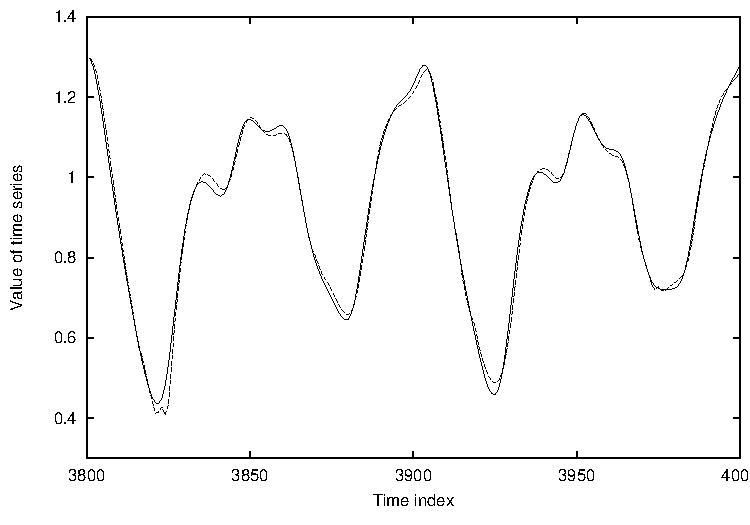
\includegraphics[width=7.5cm]{figura.pdf}
\end{center} 
\caption{Los comentarios de las figuras van debajo.} 
\label{fig:curva} 
\end{figure} 

Si quieres poner varias sub-figuras dentro de una misma figura, puedes usar el
paquete \verb+subfig+, como en la Fig.\ref{fig:subfig} (incluye Figs.~\ref{subfig:a} y \ref{subfig:b}).

\begin{figure}[ht]
    \centering
    \subfloat[Logo Sarteco]{\label{subfig:a}
    
\includegraphics[width=0.4\linewidth]{Sarteco}%
    }
    \hfill
    \subfloat[Logo Jornadas]{\label{subfig:b}
    
\includegraphics[width=0.4\linewidth]{Jornadas}%
    }
    \caption{Algunos logos.}
    \label{fig:subfig}
    \end{figure}

\begin{table}[htb]
\caption{Ejemplo de tabla. El comentario se sitúa al comienzo de la
definición de la tabla.}
\begin{center}
{\footnotesize
\begin{tabular}{|c||c|c|}\hline
N. Proc. & t  & e   \\\hline\hline
10       & 50 & 0.5 \\\hline
20       & 25 & 0.7 \\\hline
\end{tabular}
}
\end{center}
\end{table}

Incluya sus figuras preferiblemente usando ficheros en formato {\tt .pdf} en
blanco y negro o tonos de gris (el fondo debe ser siempre blanco). 

\begin{figure*}[!t]
    \centering
    \begin{minipage}{0.9\linewidth}
    {\footnotesize
    \begin{lstlisting}[language=Python]
def XCM2(events):
    n_events = len(events) (*@\label{lin:xcm-a}@*)

    Corr_max = zeros((n_events,n_events))
    Lag_max = zeros((n_events,n_events))
    Corr_min = zeros((n_events,n_events))
    Lag_min = zeros((n_events,n_events))(*@\label{lin:xcm-b}@*)

    for i in range(n_events):(*@\label{lin:xcm-i}@*)
        for j in range(i, n_events):
            xcorrij = xcorr(events[i], events[j], 250, full_xcorr=True) (*@\label{lin:xcm-c}@*)
            #Returns index and CC[i] for max(abs(CC[i])) --including negative values--
            Lag_min[i,j] = xcorrij[0](*@\label{lin:xcm-d}@*)
            Corr_min[i,j] = xcorrij[1]
            if xcorrij[1]<0.:
                #Return highest positive CC[i] and index (xcorrij[2] contains CC)
                Lag_max[i,j], Corr_max[i,j] = xcorr_max(xcorrij[2],abs_max=False)
            else:
                Lag_max[i,j] = xcorrij[0]
                Corr_max[i,j] = xcorrij[1](*@\label{lin:xcm-e}@*)

    return Corr_max, Lag_max, Corr_min, Lag_min
    \end{lstlisting}
    }
    \end{minipage}
    \caption{Código de ejemplo en python.}
    \label{fig:originalCode}
    \end{figure*}

En la Figura~\ref{fig:originalCode} se muestra un ejemplo de uso de \verb+\lstlisting+ para insertar un bloque de código. En este ejemplo el código es Python, pero se puede cambiar el ``Syntax Highlighting'' cambiando el argumento \verb+language+, por ejemplo \verb+[language=C]+. Puedes hacer referencia a las líneas de código etiquetadas con \verb+(*@\label{lin:tu-etiqueta}@*)+, como por ejemplo las líneas~\ref{lin:xcm-a}-\ref{lin:xcm-b} del código.




%!TEX root = main.tex
\section{Problemas de espacio}

Se recomienda a los autores que usen la Hoja de Estilo {\tt Jornadas.cls} que
revisen con cuidado aquellos detalles más susceptibles de generar errores al
procesar con \LaTeX, especialmente en lo que se refiere a mensajes del tipo
``underfull hbox'' u ``overfull hbox'' (o vbox). Éstos vienen casi siempre
unidos a problemas para ajustar texto u otros elementos como figuras o tablas a
la anchura y/o altura de columna de la Hoja de Estilo. La salida del proceso
\LaTeX{} le indicará la causa del problema y un número de línea aproximado del
fichero fuente en la que se ha podido producir.

En cualquier caso, no intente cambiar las definiciones de márgenes de la Hoja de
Estilo o de la plantilla de ejemplo para resolver los problemas de ajuste de
espacio. Intente alguna otra alternativa y si no resuelve el problema, consulte
con nuestra dirección de soporte para autores: {\tt js@jornadassarteco.org}.
%!TEX root = main.tex
\section{Resultados experimentales}

A la espera de resultados experimentales.


\begin{figure}[!t]
    \centering
    \begin{minipage}{\linewidth}
    {\footnotesize
    \begin{lstlisting}[language=TeX]
\documentclass[twocolumn,twoside]{Jornadas}  

\begin{document} 
    
\title{Usando la hoja de estilo ...} 
    
\author{Uno \thanks{Una Univ.}
        y Otro \thanks{Otra Univ.}} 
\maketitle
\markboth{}{}
\pagestyle{empty} 
\thispagestyle{empty}
    
\begin{abstract} 
Este artículo ... 
\end{abstract} 
    
\begin{keywords} 
Hoja de estilo, ... 
\end{keywords} 
    
\section{Introducción} 
\PARstart{L}{a} hoja de estilo ... 
    
\begin{table}[htb] 
\caption{Ejemplo de tabla...} 
\begin{center}{\tt 
    \begin{tabular} 
    ... 
    \end{tabular}} 
\end{center} 
\end{table} 
... 
\begin{figure}[htb] 
\begin{center} 
    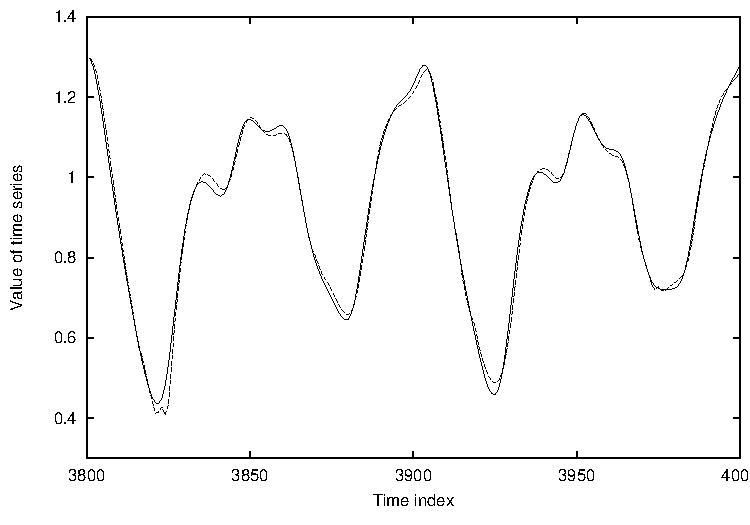
\includegraphics[width=7.5cm]{figura.pdf} 
\end{center} 
\caption{Comparación de la serie ...} 
\label{fig:curva}\end{figure} 
... 

\bibliographystyle{Jornadas} 
\bibliography{fichero.bib} 
\end{document} 
    \end{lstlisting}
    }
    \end{minipage}
    \caption{Entrada para producir este artículo. Este comentario a la figura 
    va al final de la definición de la figura.}
    \label{fig:programa}
    \end{figure}
%!TEX root = main.tex
\section{Conclusiones}

Y esto es todo. Esperamos haber ayudado con esta plantilla a la que puedes
contribuir haciendo Pull Request de este respositorio github: \url{}.


\section*{Agradecimientos}

Añadir en esta sección no numerada los posibles agradecimientos a proyectos,
instituciones o personas. Por ejemplo: El presente trabajo ha sido financiado
mediante  el proyecto xxxx-xxxxx-xxx. 

%Comenta la línea \nocite para que sólo se incluyan en las referencias
%las entradas que esté referenciadas en el texto con \cite{}
\nocite{*}
\bibliographystyle{Jornadas}
\bibliography{biblio}

\end{document}

